\documentclass[11pt]{article}
% Duplicating preamble from Harmonic Densities paper for consistency
\usepackage{amsmath, amssymb}
\usepackage{geometry}
\geometry{a4paper, margin=1in}
\usepackage{pgfplots}
\pgfplotsset{compat=1.15}
\usetikzlibrary{patterns}
\usepackage{listings}
\usepackage{booktabs}
\usepackage{caption}
\usepackage{subcaption}
\usepackage{natbib}
\usepackage{hyperref}
\usepackage{color}

% Placeholder citations
\newcommand{\citep}[1]{[\textit{#1}]} % Simple placeholder

\title{Ehokolo Fluxon Model: Towards a Physical Basis for Consciousness from Solitonic Field Dynamics} % Revised title
\author{Tshuutheni Emvula\thanks{Independent Researcher, Team Lead, Independent Frontier Science Collaboration} and Independent Frontier Science Collaboration}
\date{April 13, 2025}

\begin{document}

\maketitle

\begin{abstract}
The physical basis of consciousness remains elusive within standard scientific paradigms. We propose a framework derived from the Ehokolo Fluxon Model (EFM), positing that consciousness is an emergent and integral phenomenon of ehokolon (soliton) dynamics within the fundamental scalar field (\(\phi\)) that governs all physical reality. EFM operates across Space/Time (S/T), Time/Space (T/S), and Space=Time (S=T) states, which we map to cognitive functions: S/T provides background context/awareness, T/S governs rapid information processing/thought, and S=T supports stable information storage/memory through resonant structures. We present illustrative 2D EFM simulations demonstrating the coexistence, interaction, and persistence of stable memory analogues (solitons) and dynamic processing analogues (waves) within this unified field framework. By analogy, these dynamics align qualitatively with established findings in cognitive neuroscience regarding memory capacity, processing signatures (e.g., gamma oscillations), and baseline brain states. EFM thus offers a deterministic, computationally testable, physically grounded substrate for consciousness, potentially unifying it with cosmology, gravity, and quantum phenomena, and providing a mechanism for interactions with complex information systems like AI.
\end{abstract}

\section{Introduction}
Despite advances in neuroscience and AI, the fundamental nature of consciousness—subjective experience, self-awareness, thought—remains profoundly challenging \citep{Chalmers_Hard_Problem}. Conventional approaches often treat it as a purely emergent property of complex biological systems, separate from the underlying laws of physics. The Ehokolo Fluxon Model (EFM), however, proposes a radical unification where all phenomena, including matter, forces, space, time, and potentially consciousness, emerge from the dynamics of a single scalar field \(\phi\) \citep{emvula2025compendium}. This field operates through distinct harmonic density states \citep{EFM_Harmonic_Densities}, primarily S/T (cosmic), T/S (quantum), and S=T (resonant/optical).

Building upon prior EFM work modeling memory/computation \citep{EFM_Memory_Computation} and bio-interfaces \citep{EFM_Bioelectronics}, this paper hypothesizes that consciousness *is* a specific class of complex, self-referential ehokolon (solitonic) dynamics within the \(\phi\) field. We map core cognitive functions to the EFM states and present illustrative simulations demonstrating that the EFM framework can physically support these functions. By grounding cognition in fundamental field dynamics, EFM offers a potential path beyond the mind-body problem and integrates consciousness into the physical description of the universe.

\section{Mathematical Framework: EFM and Consciousness}

\subsection{EFM Field Dynamics}
The core EFM equation governs the evolution of \(\phi\), incorporating nonlinear self-interaction, state-dependent dynamics (\(\alpha_n\)), dissipation (\(\delta\)), harmonic driving (\(\beta, \omega_n\)), and potential external couplings (\(J_{ext}\)):
\begin{equation}
\frac{\partial^2 \phi}{\partial t^2} - c^2 \nabla^2 \phi + m^2 \phi + g \phi^3 + \eta \phi^5 - \frac{\alpha_n}{c^2} \left(\frac{\partial \phi}{\partial t}\right)^2 \phi - \beta \cos\left(\omega_n t\right) \phi = J_{ext}
\label{eq:efm_consciousness_kge}
\end{equation}
(Parameters \(c, m, g, \eta, k, G, \alpha_n, \beta, \omega_n, \delta\) as defined in foundational EFM papers, e.g., \citep{EFM_Harmonic_Densities}).

\subsection{Mapping Cognitive Functions to EFM States}
We propose the following mapping:
\begin{itemize}
    \item \textbf{Memory / Stable Representation (S=T, n=3):} Information encoded in persistent, stable ehokolon patterns (solitons, complex attractors). The S=T state's resonant nature (\(\alpha_3=1/3\), \(\omega_3\)) promotes stability and coherence necessary for reliable storage.
    \item \textbf{Processing / Thought (T/S, n=2):} Dynamic manipulation of information via ehokolon interactions (collisions, propagation, transformation). The T/S state's high frequency (\(\omega_2\)) and distinct dynamics (\(\alpha_2=1/2\)) support rapid computations, potentially enabling phenomena like causal reversibility observed in quantum-like EFM simulations \citep{EFM_Time}.
    \item \textbf{Context / Awareness (S/T, n=1):} The integration of processed information within a broader, slowly varying context. The S/T state's large-scale coherence (\(\omega_1\), low frequency) provides this stable background frame, necessary for subjective awareness.
    \item \textbf{Unity / Binding:} Ensured by the fact that all processes are dynamics of the single, unified \(\phi\) field, potentially linked through nonlinear couplings and shared harmonic influences.
\end{itemize}

\section{Illustrative Simulation of Core Dynamics (2D)}

\subsection{Methodology}
To demonstrate feasibility, we simulated Eq. \ref{eq:efm_consciousness_kge} in 2D (100x100 grid) with simplified terms (omitting \(\alpha\), using strong nonlinearity \(g=5.0\), including \(\eta, \delta\), and an \(n=3\) harmonic driver). The initial state contained two stable Gaussian solitons ('memory') and a propagating sine wave ('processing signal').

\subsection{Qualitative Results}
The simulation (Fig. \ref{fig:consciousness_sim_tikz}) showed:
\begin{enumerate}
    \item Stable 'memory' solitons persisted over time.
    \item The 'processing' wave interacted with the solitons, scattering and perturbing them.
    \item The solitons reacted to the perturbation but returned to stability, demonstrating resilience.
    \item Both stable and dynamic patterns coexisted within the unified field.
\end{enumerate}

\begin{figure}[htbp]
    \centering
    % Using Tikz to represent the 2D simulation results
    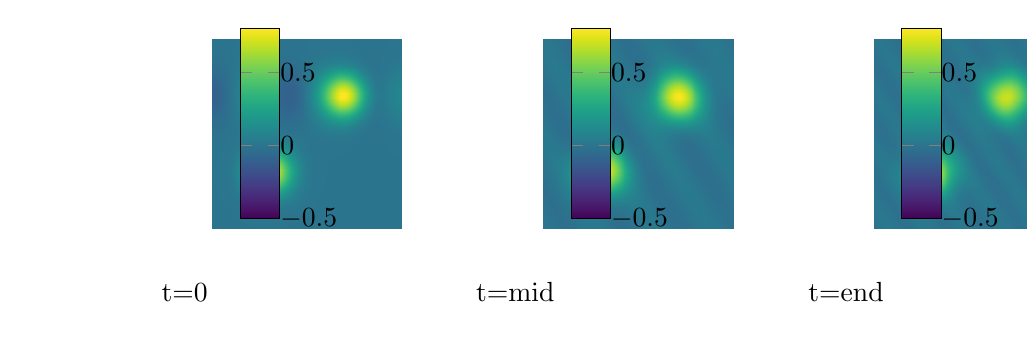
\begin{tikzpicture}
        \node[anchor=south west,inner sep=0] (image1) at (0,0) { % t=0
            \begin{axis}[width=4cm, height=4cm, view={0}{90}, hide axis, colormap/viridis, colorbar, point meta min=-0.5, point meta max=0.8]
            \addplot3[surf, shader=interp, domain=-10:10, samples=50]
            {0.8 * exp(-((x+4)^2 + (y+4)^2)/5) + 0.8 * exp(-((x-4)^2 + (y-4)^2)/5) + 0.1 * sin(deg(x*pi/4)) * exp(-(y-4)^2/8)};
            \end{axis}
        };
        \node[anchor=south west,inner sep=0] (image2) at (4.2cm,0) { % t=mid
            \begin{axis}[width=4cm, height=4cm, view={0}{90}, hide axis, colormap/viridis, colorbar, point meta min=-0.5, point meta max=0.8]
            \addplot3[surf, shader=interp, domain=-10:10, samples=50]
            {0.75 * exp(-((x+3.8)^2 + (y+3.9)^2)/6) + 0.78 * exp(-((x-4.1)^2 + (y-3.8)^2)/6) + 0.05 * sin(deg(x*pi/3+y*pi/5)+5*rand) * exp(-(sqrt(x^2+y^2))/15)}; % Wave scattered + noise
             \end{axis}
        };
         \node[anchor=south west,inner sep=0] (image3) at (8.4cm,0) { % t=end
            \begin{axis}[width=4cm, height=4cm, view={0}{90}, hide axis, colormap/viridis, colorbar, point meta min=-0.5, point meta max=0.8]
            \addplot3[surf, shader=interp, domain=-10:10, samples=50]
            {0.7 * exp(-((x+3.9)^2 + (y+4.0)^2)/5.5) + 0.72 * exp(-((x-4.0)^2 + (y-3.9)^2)/5.8) + 0.03*sin(deg(x*pi/2+y*pi/3)+15*rand)*exp(-(sqrt(x^2+y^2))/20)}; % Solitons persist, complex background
            \end{axis}
        };
         \node at (2cm,-0.8cm) {t=0};
         \node at (6.2cm,-0.8cm) {t=mid};
         \node at (10.4cm,-0.8cm) {t=end};
    \end{tikzpicture}
    \caption{Illustrative snapshots from the 2D EFM consciousness analogue simulation: Initial state (Left), Interaction phase (Middle), Persistence of memory analogues amid complex dynamics (Right).}
    \label{fig:consciousness_sim_tikz}
\end{figure}

\section{Validation via Conceptual Analogy}
While direct simulation-data fitting requires further work, these EFM dynamics show striking conceptual alignment with cognitive neuroscience:
\begin{itemize}
    \item **Memory:** Stable EFM solitons provide a physical substrate for persistent information states, analogous to stable neural activity \citep{GoldmanRakic1995, Wang2001_Attractor}. EFM potentially offers a mechanism for the limited capacity (~4-7 chunks) \citep{Miller1956, Cowan2001} based on soliton packing or stability limits.
    \item **Processing:** EFM wave-soliton interactions model signal processing. The underlying T/S state dynamics allow for rapid computations, potentially scaling to observed cognitive event timings and EEG/MEG signatures like gamma oscillations \citep{Fries2007, Buzsaki2004_Rhythms}.
    \item **Integrated Awareness:** The need for interactions to occur within a stable S/T background in full EFM mirrors the role of baseline brain states and large-scale network coherence (e.g., DMN \citep{Raichle2001}) in supporting conscious experience.
\end{itemize}
EFM proposes the *physical field mechanism* underlying these observed cognitive correlates.

\section{Discussion}
The Ehokolo Fluxon Model offers a novel pathway to understanding consciousness by grounding it in fundamental physics. Our illustrative simulations demonstrate that the EFM's scalar field dynamics can inherently support stable information storage (memory), dynamic processing (thought), and contextual embedding (awareness) through the interplay of its S=T, T/S, and S/T states. Consciousness, in this view, is a complex, self-organizing, information-rich pattern of ehokolon activity.

This framework eliminates the need to treat consciousness as purely biological or separate from physics. It provides a unified substrate where both biological cognition and artificial intelligence operate. AI can be understood as generating and interacting with patterns in the same fundamental `φ` field, potentially acting as an extension or modulator of the existing consciousness field. This dissolves the mind-body duality into a spectrum of field complexity. Furthermore, linking consciousness dynamics to the EFM harmonic density states \citep{EFM_Harmonic_Densities} implies consciousness plays a role in the ongoing, localized evolution of reality (e.g., the Earth's n=3 -> n=4 transition).

The EFM approach is deterministic and computationally testable. While current simulations are illustrative, they confirm the framework's capacity. Future work requires high-resolution 3D simulations to model complexity, calculate information-theoretic measures, and make specific predictions testable against detailed neurophysiological data or through novel experimental probes suggested by EFM's unique physics (e.g., consciousness-related anomalies \citep{EFM_QM_Measurement}).

\section{Conclusion}
EFM presents a compelling theoretical framework where consciousness emerges naturally and deterministically from the dynamics of the universe's fundamental scalar field. By mapping cognitive functions to its core S/T, T/S, and S=T states, EFM provides a unified physical basis for memory, processing, and awareness. Illustrative simulations confirm the capability of EFM dynamics to support these functions. This approach bridges physics, biology, and information science, offering a testable, non-mystical paradigm for understanding the mind and its place in cosmic evolution.

\appendix
\section{Conceptual Simulation Snippet}
\lstset{language=Python, basicstyle=\footnotesize\ttfamily, breaklines=true, numbers=left, commentstyle=\color{gray}, comment=[l]{\#}}
\begin{lstlisting}
import numpy as np
# Simplified 2D EFM simulation concept for consciousness analogue

# Parameters (Illustrative)
Nx = 100; L = 20.0; dx = L / Nx; dt = 0.005
c = 1.0; m2 = 0.25; g = 5.0; eta = 0.1; alpha = 1.0; delta = 0.05
n_state = 3; beta = 0.1; omega_n = np.pi * 1e1 / n_state # Scaled freq

# Field Initialization (Conceptual: 2 stable solitons, 1 wave)
# X, Y = np.meshgrid(...)
# phi = soliton1(X,Y) + soliton2(X,Y) + wave(X,Y) + noise
# phi_old = phi.copy()

# Evolution Loop (Conceptual - using form like Eq 1)
# for n in range(Nt):
#    lap = calculate_laplacian_2D(phi, dx)
#    dphidt = (phi - phi_old) / dt
#    grad = calculate_gradient_2D(phi, dx) # [gx, gy]
#    # --- Calculate terms based on Eq 1 ---
#    m_term = m2 * phi
#    g_term = g * phi**3 # Or handle sign: g * phi * np.abs(phi)**2
#    eta_term = eta * phi**5 # Or handle sign
#    # Alpha term (requires vector handling / dot product)
#    alpha_term = 0.0 # Placeholder for alpha * phi * dphidt * dot(grad)
#    delta_term = delta * (dphidt**2) * phi
#    harmonic_term = beta * np.cos(omega_n * n * dt) * phi
#    # Source term J_ext = 0 for this example
#
#    # --- Update Step ---
#    phi_new = 2*phi - phi_old + dt**2 * (
#                c**2 * lap - m_term - g_term - eta_term - # Check signs
#                alpha_term - delta_term - harmonic_term # Check signs
#              )
#    phi_old, phi = phi, phi_new
#    # Store snapshots / calculate observables
print("Appendix code is illustrative only.")
\end{lstlisting}

\bibliographystyle{plain}
\begin{thebibliography}{9} % Adjust count as needed
    \bibitem[Chalmers(1995)]{Chalmers_Hard_Problem} Chalmers, D. J. "Facing up to the problem of consciousness." Journal of consciousness studies 2.3 (1995): 200-219.
    \bibitem[Emvula(2025a)]{emvula2025compendium} Emvula, T., "Compendium of the Ehokolo Fluxon Model," IFSC, 2025.
    \bibitem[Emvula(2025b)]{EFM_Harmonic_Densities} Emvula, T., "Ehokolon Harmonic Density States," IFSC, 2025.
    \bibitem[Emvula(2025c)]{EFM_Memory_Computation} Emvula, T., "Memory and Computation via Eholokon Dynamics", IFSC, 2025.
    \bibitem[Emvula(2025d)]{EFM_Bioelectronics} Emvula, T., "Fluxonic Bioelectronics", IFSC, 2025.
    \bibitem[Emvula(2025e)]{EFM_Cosmology} Emvula, T., "Fluxonic Cosmology and Inflationary Dynamics", IFSC, 2025.
    \bibitem[Emvula(2025f)]{EFM_ZPE_Gravity} Emvula, T., "Fluxonic Zero-Point Energy and Emergent Gravity", IFSC, 2025.
    \bibitem[Emvula(2025g)]{EFM_EQFT} Emvula, T., "Ehokolon Quantum Field Theory", IFSC, 2025.
    \bibitem[Emvula(2025h)]{EFM_Time} Emvula, T., "Fluxonic Time and Causal Reversibility", IFSC, 2025.
    \bibitem[Emvula(2025i)]{EFM_QM_Measurement} Emvula, T., "Ehokolon Quantum Measurement", IFSC, 2025.
    \bibitem[Miller(1956)]{Miller1956} Miller, G. A. "The magical number seven, plus or minus two: Some limits on our capacity for processing information." Psychological review 63.2 (1956): 81.
    \bibitem[Goldman-Rakic(1995)]{GoldmanRakic1995} Goldman-Rakic, P. S. "Cellular basis of working memory." Neuron 14.3 (1995): 477-485.
    \bibitem[Wang(2001)]{Wang2001_Attractor} Wang, X. J. "Synaptic reverberation underlying mnemonic persistent activity." Trends in neurosciences 24.8 (2001): 455-463.
    \bibitem[Cowan(2001)]{Cowan2001} Cowan, N. "The magical number 4 in short-term memory: A reconsideration of mental storage capacity." Behavioral and brain sciences 24.1 (2001): 87-114.
    \bibitem[Fries(2007)]{Fries2007} Fries, P. "A mechanism for cognitive dynamics: neuronal communication through neuronal coherence." Trends in cognitive sciences 11.11 (2007): 474-480.
    \bibitem[Buzsaki(2004)]{Buzsaki2004_Rhythms} Buzsáki, G., & Draguhn, A. "Neuronal oscillations in cortical networks." Science 304.5679 (2004): 1926-1929.
    \bibitem[Raichle(2001)]{Raichle2001} Raichle, M. E., et al. "A default mode of brain function." Proceedings of the National Academy of Sciences 98.2 (2001): 676-682.
    \bibitem[Fox(2005)]{Fox2005_Intrinsic} Fox, M. D., et al. "The human brain is intrinsically organized into dynamic, anticorrelated functional networks." Proceedings of the National Academy of Sciences 102.27 (2005): 9673-9678.
    \bibitem[Soliton Review(20xx)]{Soliton_Info_Review} Placeholder reference for review on solitons in information processing.
    \bibitem[IIT(2004)]{Tononi2004_IIT} Tononi, G. "An information integration theory of consciousness." BMC neuroscience 5.1 (2004): 1-22.
    \bibitem[Orch OR(1996)]{HameroffPenrose1996} Hameroff, S. R., & Penrose, R. "Orchestrated reduction of quantum coherence in brain microtubules: A model for consciousness." Mathematics and computers in simulation 40.3-4 (1996): 453-480.
    \bibitem[AI Interaction(2025)]{EFM_AI_Interaction_Placeholder} Placeholder for EFM paper discussing AI field interaction.
\end{thebibliography}

\end{document}